\documentclass[
	12pt,
]{fphw}
\usepackage{xeCJK}
\usepackage{setspace}
\usepackage{subfigure}
\usepackage{mathbbol}
\usepackage{amsmath}
\usepackage{float}
\usepackage{color}
\usepackage{listings}
\usepackage[hidelinks]{hyperref}
\usepackage{minted}
\usepackage[utf8]{inputenc} % Required for inputting international characters
\usepackage[T1]{fontenc} % Output font encoding for international characters
\usepackage{mathpazo} % Use the Palatino font
\usepackage{graphicx} % Required for including images
\usepackage{booktabs} % Required for better horizontal rules in tables
\usepackage{listings} % Required for insertion of code
\usepackage{enumerate} % To modify the enumerate environment
\lstset{ %
language=python,                % choose the language of the code
basicstyle=\footnotesize,       % the size of the fonts that are used for the code
numbers=left,                   % where to put the line-numbers
numberstyle=\footnotesize,      % the size of the fonts that are used for the line-numbers
stepnumber=1,                   % the step between two line-numbers. If it is 1 each line will be numbered
numbersep=5pt,                  % how far the line-numbers are from the code
backgroundcolor=\color{white},  % choose the background color. You must add \usepackage{color}
showspaces=false,               % show spaces adding particular underscores
showstringspaces=false,         % underline spaces within strings
showtabs=false,                 % show tabs within strings adding particular underscores
frame=single,           % adds a frame around the code
tabsize=2,          % sets default tabsize to 2 spaces
captionpos=b,           % sets the caption-position to bottom
breaklines=true,        % sets automatic line breaking
breakatwhitespace=false,    % sets if automatic breaks should only happen at whitespace
escapeinside={\%*}{*)}          % if you want to add a comment within your code
}

\onehalfspacing
\title{Homework 3} % Assignment title
\author{黄嘉诚  2023311381} % Student name

\date{\today} % Due date

\institute{Tsinghua University } % Institute or school name

\class{深度学习} % Course or class name

\professor{龙明盛} % Professor or teacher in charge of the assignment

%----------------------------------------------------------------------------------------

\begin{document}

\maketitle % Output the assignment title, created automatically using the information in the custom commands above

%----------------------------------------------------------------------------------------
%	ASSIGNMENT CONTENT
%----------------------------------------------------------------------------------------

\part*{Part One: Transformer}

\section*{Task 1}

\begin{problem}
	\medskip
		\quad Construct the standard Transformer and train your model from scratch using the recommended deep learning framework. Validate your model on the valid set, and report training and validation curves. Evaluate the best model on the test set.
	\end{problem}

	
\subsection*{Solution}
补充后的注意力模块见attention.py文件,直接运行它可得
\begin{minted}{python}
self_attn_output error:  0.0001443615577231714
masked_self_attn_output error:  0.00014208846529652346
attn_output error:  0.0001246251842128651
\end{minted}
\qquad 结果非常接近0,说明注意力模块实现正确。直接运行run.py,将得到的结果绘图:
\begin{figure}[h]
	\centering  %图片全局居中
	\subfigure[训练和验证集]{
		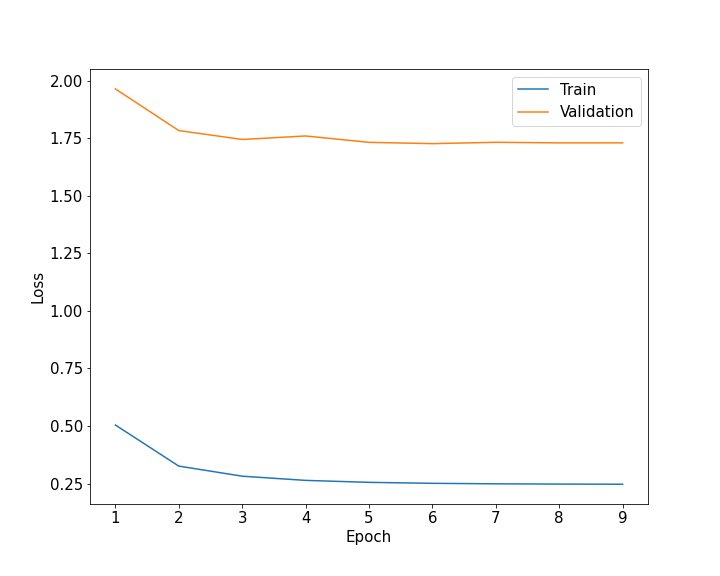
\includegraphics[width=0.48\textwidth]{train.png}}
		\subfigure[测试集]{
		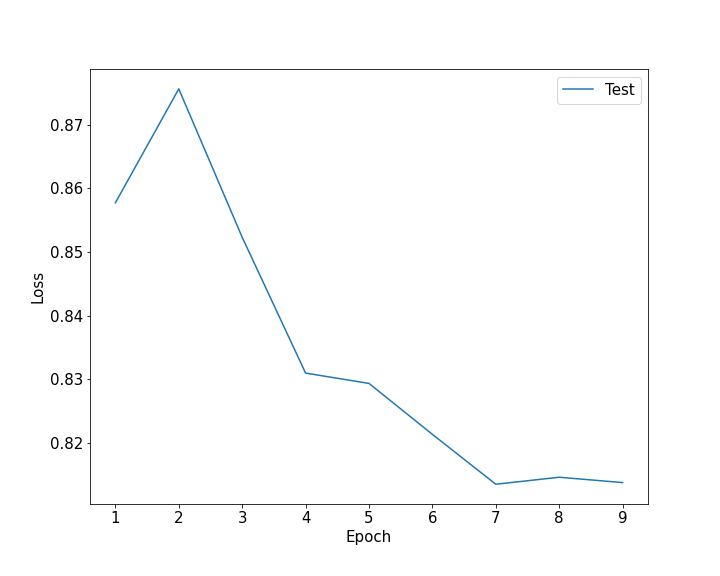
\includegraphics[width=0.48\textwidth]{test.png}}
	\caption{Transformer运行结果}
	\label{tr}
	\end{figure}
\qquad 最终在测试集上的MSE为0.8216503858566284,MAE为0.6647586226463318。



\section*{Task 2}

\begin{problem}
	\medskip
		\quad Please explain why the mask is necessary in Transformer and how it is implemented in your code.
	\end{problem}

\subsection*{Solution} 在Transformer网络中,mask技术是必须的,主要原因是为了处理自注意力机制(self-attention)时的信息泄露问题。自注意力机制允许模型在处理序列数据时关注序列中的不同位置,但在一个序列中的某个位置计算注意力时,理论上它可以看到该位置之后的所有信息。在训练过程中,为了保证模型是自回归的,需要增加mask以避免预测时模型看到待预测单元及其后面的序列。如果没有mask,那么模型将会作弊,无法学习到有效信息,泛化能力大大降低。同时,采用mask技术可以代替原始的逐个生成的自回归技术,采用矩阵计算加速了学习过程。
    


\section*{Task 3}

\begin{problem}
	\medskip
		\quad Please visualize the attention values of some typical words and check whether the Transformer can learn meaningful attention values.
	\end{problem}


\subsection*{Solution}





\section*{Task 4}

\begin{problem}
	\medskip
		\quad Please adopt an extra technique (Hint: some linear attention or sparse attention) you find in other materials to further improve your model. Please explain why you chose it, check whether it works on our given dataset, and give a convincing reason.
	\end{problem}

\subsection*{Solution}
\par
1. 优点:字母表字母少,所需参数量相应较小;避免了单词不在词表中的情形,预处理数据更方便;更适合词性变化等字母级别的任务学习。

\par
2. 缺点:字母出发需要先学会构建单词,单词中字母的组合方式非常复杂,RNN仅仅学习到这一点就很困难;字母基础的RNN更难捕捉到长程关系,因为一段话可能只有几十个单词,但字母有上百个;因此注意力机制会消耗大量内存,对模型进一步改进不利。



\part*{Part Two: Generative Adversarial Networks (GAN)}

\section*{GAN Implementation}



\subsection*{Solution} 直接运行即可,训练曲线见图\ref{gcn}。\par
1. GCN, Best Test Accuracy: 0.828, Train: 0.986, Val: 0.792;\par
2. GAT, Best Test Accuracy: 0.831, Train: 0.986, Val: 0.808;\par
3. Node2Vec, Best Test Accuracy: 0.734, Loss: 0.8247


\begin{figure}[h]
	\centering  %图片全局居中
	\subfigure[GCN]{
	\includegraphics[width=0.48\textwidth]{GCN_curves.png}}
	\subfigure[GAT]{
		\includegraphics[width=0.48\textwidth]{GAT_curves.png}}
		\subfigure[Node2Vec]{
		\includegraphics[width=0.48\textwidth]{node2vec.png}}
		\subfigure[Node2Vec(visualize)]{
		\includegraphics[width=0.48\textwidth]{visualization.png}}
	\caption{GCN,GAT与Node2Vec运行结果}
	\label{gcn}
	\end{figure}



\section*{Least Squire GAN}

\subsection*{Solution}
	

\par 选择实现DeepGCN,代码在同名文件DeepGCN.py中。参考了PyG所给实例(\href{https://github.com/pyg-team/pytorch_geometric/blob/master/examples/ogbn_proteins_deepgcn.py}{ogbn\_proteins\_deepgcn}),得到结果如图\ref{dgcn}所示,层数太大,效果反而不好。\par

Layers = 1, Best Test Accuracy: 0.741, Train: 1.000, Val: 0.716 \par

Layers = 2, Best Test Accuracy: 0.732, Train: 1.000, Val: 0.738 \par

Layers = 4, Best Test Accuracy: 0.719, Train: 1.000, Val: 0.71 \par

Layers = 8, Best Test Accuracy: 0.743, Train: 1.000, Val: 0.7 \par

Layers = 16, Best Test Accuracy: 0.746, Train: 1.000, Val: 0.752 \par

Layers = 32, Best Test Accuracy: 0.681, Train: 1.000, Val: 0.648 \par
Layers = 64, Best Test Accuracy: 0.6, Train: 1.000, Val: 0.622 \par

\begin{figure}[h]
	\centering  %图片全局居中
	\subfigure[Layers = 1]{
	\includegraphics[width=0.48\textwidth]{DeepGCN_curves_1.png}}
	\subfigure[Layers = 2]{
		\includegraphics[width=0.48\textwidth]{DeepGCN_curves_2.png}}
		\subfigure[Layers = 4]{
		\includegraphics[width=0.48\textwidth]{DeepGCN_curves_4.png}}
		\subfigure[Layers = 8]{
		\includegraphics[width=0.48\textwidth]{DeepGCN_curves_8.png}}
		\subfigure[Layers = 16]{
	\includegraphics[width=0.48\textwidth]{DeepGCN_curves_16.png}}
	\subfigure[Layers = 32]{
		\includegraphics[width=0.48\textwidth]{DeepGCN_curves_32.png}}
		\subfigure[Layers = 64]{
			\includegraphics[width=0.48\textwidth]{DeepGCN_curves_64.png}}
	\caption{GCN,GAT与Node2Vec运行结果}
	\label{dgcn}
	\end{figure}
\end{document}

\section*{Deeply Convolutional GAN}
